\subsection{Steep Parabola-shaped Branches $f_\A$ and $f_\C$}
\label{sec:setup.quad.hyper.1}

\hl{The values of the compound parameters $g_R\left(\frac{1}{4}\right)$ and $\left. \frac{d}{dx} g_R\left(x\right) \right|_{x = \frac{1}{2}}$ are fixed as described previously in} \Cref{sec:setup.quad.hyper.params}.
\hl{In this section, the values of the parameters of the function $g_L$ are set to $a_L = 8$ and $b_L = -1$ to get steep, shifted parabola-shaped branches $f_\A$ and $f_\D$, as one can see in the cobweb diagrams in} \Cref{fig:setup.quad.hyper.1.cobwebs}.
Scanning the periods for \hl{reasonable} values of $\alpha = g_R\left(\frac{1}{4}\right)$ and \hl{the parameter} $\beta = c_L$ results in \Cref{fig:setup.quad.hyper.1.period}.
The \hl{reasonable} values for $\alpha = g_R\left(\frac{1}{4}\right)$ are larger than $\frac{1}{4}$ to keep the parabola above the bisector $y = x$ and smaller than $\frac{1}{2}$ to keep the value \hl{of the model function} at the left borders of the branches $f_\B$ and $f_\D$ below the value \hl{of the model function} at the right borders.
For the specified values of $a_L$ and $b_L$, the reasonable values for $\beta = c_L$ are smaller than $0.22$ to not map the points directly onto the branch $f_\C$ from the branch $f_\A$.
To keep the parabola above the bisector $y = x$, the values for $\beta$ should also be larger than $0.12$.

\hl{
	With the newly chosen fixed parameters and the new compound parameters, this model imitates the shape of the original model function well still.
}
\hl{The parameter $c_L$ is also still varied and this emulates the effects of $\chi_0$ on the branches $F_\A$ and $F_\C$ of the original model function well, as described in the previous section,} \Cref{sec:setup.quad}.
\hl{
	The other varied parameter is the compound parameter $g_R\eft(\frac{1}{4}\right)$.
	For brevity the varied parameters are named $\alpha = g_R\eft(\frac{1}{4}\right)$ and $\beta = c_L$.
	Varying the parameter $\alpha$ is a major improvement for emulating the effects of $E_0$ on the branches $F_\B$ and $F_\D$ of the original model function.
	Increasing $\alpha$ primarily increases the values of the model function on the left sides of the branches $f_\B$ and $f_\D$ and keeps the values on the right sides the same.
	It also moves the local minima of those branches to the left and decreases the value of the model function at those points, just as the parameter $E_0$ did to the original model function.
}

\begin{figure}
	\centering
	\includegraphics[width=0.6\textwidth]{40_Quadratic_fittingR/2D_Period_Whole/result.png}
	\caption[2D scan of the periods of the quadratic model with hyperparameters]{
	2D scan of the periods of the piecewise quadratic model with compound parameters $g_R\left(\frac{1}{4}\right), g_R\left(\frac{1}{2}\right),$ and $\left. \frac{d}{dx} g_R\left(x\right) \right|_{x = \frac{1}{2}}$.
	The parameters $a_L = 8, b_L = -1, g_R\left(\frac{1}{4}\right) = 0.525,$ and $\left. \frac{d}{dx} g_R\left(x\right) \right|_{x = \frac{1}{2}} = 1.2$ are fixed.
	The parameters $\alpha = g_R\left(\frac{1}{4}\right)$ and $\beta = c_L$ are varied in the ranges $[0.25, 0.5]$ and $[0.12, 0.22]$, respectively.
	The points $A, B,$ and $C$ mark the parameter values used for the cobweb diagrams in \Cref{fig:setup.quad.hyper.1.cobwebs}.
	Also, the numbers at the top indicate the period associated with some parameter regions.
	}
	\label{fig:setup.quad.hyper.1.period}
\end{figure}

\begin{figure}
	\centering
	\begin{subfigure}{0.3\textwidth}
		\centering
		\includegraphics[width=\textwidth]{40_Quadratic_fittingR/Cobweb_A/result.png}
		\caption{At Point $A$}
		\label{fig:setup.quad.hyper.1.cobweb.A}
	\end{subfigure}
	\begin{subfigure}{0.3\textwidth}
		\centering
		\includegraphics[width=\textwidth]{40_Quadratic_fittingR/Cobweb_B/result.png}
		\caption{At Point $B$}
		\label{fig:setup.quad.hyper.1.cobweb.B}
	\end{subfigure}
	\begin{subfigure}{0.3\textwidth}
		\centering
		\includegraphics[width=\textwidth]{40_Quadratic_fittingR/Cobweb_C/result.png}
		\caption{At Point $C$}
		\label{fig:setup.quad.hyper.1.cobweb.C}
	\end{subfigure}
	\caption[Cobwebs of the first piecewise quadratic model with hyperparameters]{
	Cobweb diagrams at three parameter values of $\alpha = g_R\left(\frac{1}{4}\right)$ and $\beta = c_L$ in the piecewise quadratic model with hyperparameters.
	The other parameters are fixed as $a_L = 8, b_L = -1, g_R\left(\frac{1}{2}\right) = \frac{1}{2} + \frac{1}{40}$, and $\left. \frac{d}{dx} g_R(x) \right|_{x = \frac{1}{2}} = 1 + \frac{1}{5}$.
	The parameter values are marked in \Cref{fig:setup.quad.hyper.1.period}.
	(a) shows the cycle $\Cycle{\A^4\B^5\C^4\D^5}$ at point $A$ \hl{where $\alpha = 0.42$ and $\beta = 0.1525$},
	(b) shows the cycle $\Cycle{\A^3\B^6\D^3\C^6}$ at point $B$ \hl{where $\alpha = 0.385$ and $\beta = 0.1675$},
	and (c) shows the cycle $\Cycle{\A^2\B^7\C^2\D^7}$ at point $C$ \hl{where $\alpha = 0.385$ and $\beta = 0.1675$}.
	}
	\label{fig:setup.quad.hyper.1.cobwebs}
\end{figure}

\Cref{fig:setup.quad.hyper.1.period} \hl{shows a 2D scan of the periods associated eith parameter regions in the specified parameter reange for $\alpha$ and $\beta$}.
\hl{
	At the top, some periods are annotated.
	One can see that in the scan there are sequences of parameter regions that are associated with the same period.
	These sequences are next to each other, where each sequence is associated with a period that is two numbers higher than the period associated with the parameter region sequence right to it.
}
\hl{This is similar to the \gls{pi} that can be observed in the original model, as described in} \Cref{sec:state.og.dynamics}.
\hl{
	One difference is that the sequences in the original model were connected and formed chains.
}

\Cref{fig:setup.quad.hyper.1.cobwebs} \hl{shows cobweb diagrams for different parameter values along the sequence of parameter regions associated with the period $18$}.
\hl{These parameter values are marked with points in} \Cref{fig:setup.quad.hyper.1.period}.
\Cref{fig:setup.quad.hyper.1.cobweb.A} \hl{shows the cycle at the point $A$ with the symbolic sequence $\A^4\B^5\C^4\D^5$}.
\Cref{fig:setup.quad.hyper.1.cobweb.B} \hl{shows the cycle at the point $B$ with the symbolic sequence $\A^3\B^6\C^3\D^6$}.
\hl{
	Notice that the cycle at point $B$ has one point less on the branches $f_\A$ and $f_\C$ each than the cycle at point $A$, while it has one point more on the branches $f_\B$ and $f_\D$ each.
	It is as if two points, one of each of the branches $f_\A$ and $f_\C$, moved to the next branch from one parameter region of the sequence to the next.
}
\Cref{fig:setup.quad.hyper.1.cobweb.C} \hl{shows the cycle at the point $B$ with the symbolic sequence $\A^2\B^7\C^3\D^7$}.
\hl{
	Again, two points, one of each of the branches $f_\A$ and $f_\C$, moved to the next branch from the parameter region with point $B$ to the parameter region with the point $C$.
}
\hl{This is also very similar to the behavior of the original model, where two points, one of each of the branches $F_\A$ and $F_\C$, moved to the next branch each along the chain of parameter regions associated with the same period, as described in} \Cref{sec:state.og.dynamics}.
\hl{
	Besides that the sequences of parameter region associated with the same period are not connected here, there is another difference to the behavior of the original model.
	In the original model there are ``type B'' parameter regions between the ``type A'' parameter regions of a chain of parameter regions with the same period.
	To reiterate, ``type A'' parameter regions are associated with a single symmetric cycle.
	These are the parameter regions, one can observe in this case also.
	Between two ``type A'' parameter regions there is a parameter region that is associated with two coexisting asymmetrical twin cycles, called ``type B'' parameter regions.
	These ``type B'' parameter regions are missing in this case.
}
